	The main objective of the project is to build an automatic emotion recognizer from children's speech using the more recent I Vector and DNN approach. The objective can be broken down to three secondary objectives; understanding the data to be used in the project, extracting the features required for the neural network and building and optimizing the neural network. This section's structure mirrors the objective pathway.
\section{PF Star English}
	The PF Star Children's Speech corpus was used in this project (Batliner et. al 2005). The corpus was designed to be cross lingual with the same experiments used to collect both German and English data. The AIBO experiment was designed to elicit and record via a microphone natural emotions from children (Batliner et. al 2004).
	
	% is this needed?
	
	The experiment is described as a ``Wizard-of-Oz scenario." Children were tasked with guiding a Sony AIBO robot, a dog-like robot, through a maze while fulfilling objectives. No specific instruction were given to the children besides speaking to AIBO as if it were a friend. The children were led to believe they had control over AIBO's actions, however AIBO was secretly controlled by a human operator unbeknownst to the children. Two experimental conditions were outlined; experiment E1 has the operator input instructions based on the child's commands as best as possible, emulating a high performance speech recognition system. Experiment E2, on the other hand, had the operator input a ``fixed, pre-determined sequence of actions" which takes no account of the child's commands, emulating a low performance speech recognition system. The children completed both experiments, E1 and E2, in that order, and told they were using two alternative systems.
	
\subsection{File Details}
	30 children between ages 4 and 14, inclusive, took part in both experiments. A total of 8.5 hours of recordings is provided, but only just over 1.5 hours remains once the silence, pauses and unintelligible speech are removed. The audio files were named as $nX$ where $n$ is a number between 1 and 31 indicating the child and $x$ is a letter indicating the experiment, A for E1 and B or E2. Some files were missing, corrupted or lacking labels; these have been excluded from the project. The audio files contained two audio channels from different microphones; only audio from channel one was used to avoid errors that could result from mismatched audio quality.
	
\subsection{Labeling Details}
	The corpus originally classified utterances into one of eleven emotion classes. However, due to sparsity of members in some classes, this was later revised to six emotion classes, as seen in Table \ref{classesweight}. The english data was labeled by three listeners. All three responses are available in the label files. Techniques can be used to either average, randomly select or throw away unequal labels. This project uses six emotion classes to reduce the impact of lacking data in some emotional classes. Utterances without a unanimous label are labeled randomly from the three choices. There are a total of \textbf{5302} available labeled utterances divided according to Table \ref{classesweight}.
	
	\begin{table}[hbt]
		\caption{Emotion classes sample weight}
		\centering
		\begin{tabular}{|c|c|c|}
			\hline
			Emotion Class & Sample Size & Weight \\ \hline
			Angry         & 326         & 0.062  \\ \hline
			Joyful        & 10          & 0.001  \\ \hline
			Motherese     & 38          & 0.007  \\ \hline
			Emphatic      & 576         & 0.109  \\ \hline
			Neutral       & 4338        & 0.819  \\ \hline
			Other         & 14          & 0.002  \\ \hline
		\end{tabular}
	\label{classesweight}
	\end{table}

\section{Feature Extraction}
	The feature vector used for classification algorithms in this project was the I Vector. Several steps, illustrated in Figure \ref{fig:ivecproc}, were taken to produce these vectors. MATLAB was used to convert the audio files into usable features; additionally, the MSR Identity Toolkit by (Sadjadi et. al 2013) contained functions used for UBM, I Vectors and Linear Discriminant Analysis (LDA) calculations.
	\begin{figure}[!htb]
		\center{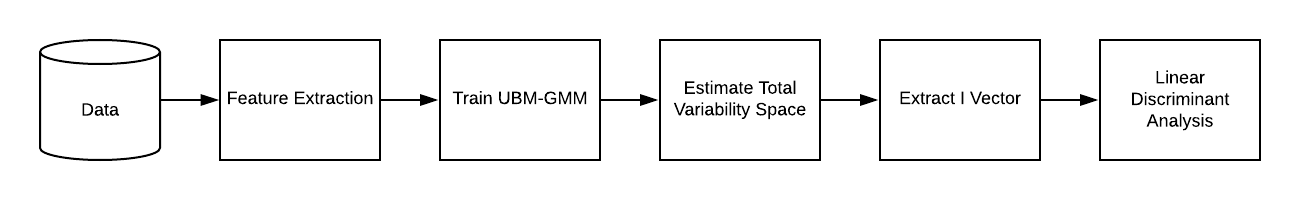
\includegraphics[width=16cm]
			{ivecproc}}
		\caption{\label{fig:ivecproc} I Vector Extraction Steps}
	\end{figure}

\subsection{MFCC}
	The audio file contains all utterances for a specified child and experiment. MFCC extraction is applied to each utterance, so the audio file is divided into segments wherein each segment matches a label. The following steps are applied to each utterance to obtain an MFCC feature vector.
	\begin{enumerate}
		\item Frame the utterance into shorter frames (20ms to 30ms) with some overlap and apply a windowing function. Hamming window was used.
		\item Take the Discrete Fourier Transform (DFT)  of the signal to convert it into the frequency domain. This is done using the \verb|stft(...)| function in MATLAB's Signal Processing library.
		\item Apply 26 triangular filter banks to the DFT output as seen in Figure \ref{fig:filterbanks}. The triangular filters match the non-linear human perception by covering a smaller area in smaller frequencies and vice versa. The log is taken of the energy in each filter.
					\begin{figure}[!htb]
			\center{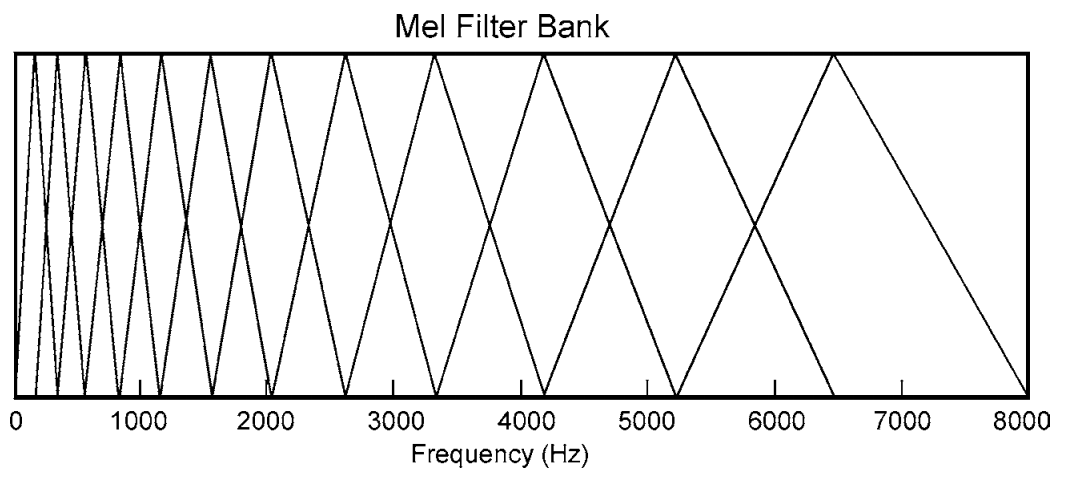
\includegraphics[width=9cm]
				{filterbanks}}
			\caption{\label{fig:filterbanks} Mel Filterbanks applied to a power spectrum of a signal}
		\end{figure}
		\item Take the Discrete Cosine Transform (DCT) of the previous output. DCT compresses the data into, usually, 26 coefficients for the frame. The upper half are thrown out, resulting in 13 coefficients.
		\item Additionally, the delta and delta-delta of the coefficients can also be calculated. MFCC coefficients contain only data from the frame analyzed; however information can also be contained with how the frames change. The delta and delta-delta are taken for this purpose.
	\end{enumerate}

	All steps after DFT are completed in the MATLAB function \verb|mfcc(...)|, outputting a 40 dimensional vector containing the 13 coefficients, deltas and delta-deltas and the log energy of the entire frame. The entire MFCC extraction process is done in the project using the custom \verb|extract_mfcc(...)| function.
	
	Following MFCC extraction, a UBM is calculated using the \verb|gmm_em(...)| function provided in the MSR Toolkit. The UBM is created using the EM algorithm and contains a user-defined $n$ components. This parameter is a target for optimization.

\subsection{I Vectors}
	To generate I Vectors, the total variability (TV) space must first be estimated. Assuming a simple factor analysis model of the form:
	\begin{equation}
		M = m + T . x
	\end{equation}
	where $M$ is the GMM Supervector, $m$ is the UBM Supervector, $T$ is the TV space, and $x$ is the I Vector. The process is to randomly initialize a $T$ matrix and compute $x$. Using a maximum likelihood estimate algorithm with the UBM, $T$ can then be recalculated. This process is computationally demanding especially at large dimensions for $T$.
	
	The function \verb|train_tvspace(...)| is provided by the MSR Toolkit to estimate $T$. The dimension of $T$ is user defined and a target for optimization. Once TV space is estimated, extracting the I Vector is simply calculating $x$. This is done in the MSR Identity Toolkit with the provided function \verb|extract_ivector(...)|
	
\subsection{Linear Discriminant Analysis}
	I Vectors can be dimensionally reduced further using Linear Discriminant Analysis (LDA). LDA projects data onto a lower-dimensional vector space such that the ratio of the between-class distance to the within-class distance is maximized. The dimension of LDA reduced data is $n-1$, where $n$ is the number of distinct classes in the data. Six emotion classes are used in this project, so the final sized feature vector is 5 dimensions in size obtained by reducing the I Vectors with the LDA function provided by the MSR Identity Toolkit.  
	
	\begin{figure}[!htb]
		\center{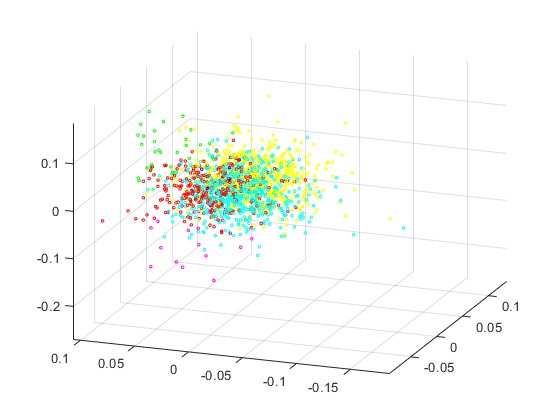
\includegraphics[width=7cm]
			{3dlda}}
		\caption{\label{fig:3dlda} First 3 dimensions of 5D LDA reduced I Vectors}
	\end{figure}

	LDA has the advantage of visualizing data in its most linearly separable dimensions. Figure \ref{fig:3dlda} presents a three dimensional plot of the LDA reduced I Vectors. Although there is some overlap between some classes, others, such as the green class, are in separate clusters. This is shown in more detail in the Results section of the paper.
\section{Automatic Classification}
\subsection{Evaluation Metric}
	The evaluation metric used in the project is Unweighted Average Recall (UAR). For each utterance $x_i$ belonging to emotion class $C_n$, $x_i$ can either be classified correctly as $C_n$ or incorrectly as another class $C_m$. These are referred to as true positive (TP) or false negative (FN), respectively. Recall (R) for class $C_n$ is defined as
	\begin{equation}
	R_n = \frac{TP_{C_n}}{TP_{C_n} + FN_{C_n}}
	\end{equation}
	and unweighted average recall for $n$ classes is defined as
	\begin{equation}
	UAR =  \frac{1}{n} \sum_{1}^{n} R_n
	\end{equation}
	
	UAR is useful for its fast computability, equal weighting of imbalanced classes and commonality in other research often using it allowing comparisons to be made with said research. During its calculation per class accuracy is also calculated, so more insight is available on the classifier should it be needed.
	
	Originally the weighted average recall (WAR) metric was considered as the primary evaluation metric. However it was prone to issues UAR was not. WAR is calculated similarly to UAR but requires class weight. The weight $w$ of each class $C_n$ is seen in Table \ref{classesweight}, and were calculated as follows.
		\begin{equation}
		w_n = \frac{i_{C_n}}{i}
		\end{equation}
	where $i_{C_n}$ is the total number of labeled utterances for emotional class $C_n$ and $i$ is the total number of utterances in all classes. WAR is calculated as follows.
	\begin{equation}
	WAR = \sum_{1}^{n} w_n * R_n
	\end{equation}
	
	WAR shares similar positives to UAR;  fast computatability and common in experiments. WAR, however, prioritizes classes with a larger ratio in the data. When recognizing emotions, the objective is to recognize each emotion correctly regardless of rarity, so a step to handle the imbalance of data in the project was to favor UAR as an evaluation metric.
\subsection{Baseline Classifiers}
	Nearest neighbor classification is used as the baseline classifier in this project. The first step to nearest neighbor is to find the mean vector $\mu_n$ of each emotional class $C_n$. For an n-dimensional vector, the mean vector will be n-dimensional. With test input data, a similarity measure $sim_{ni}$ is calculated between a feature vector $x_i$ and mean vectors $\mu_n$. The mean vector with the lowest $sim_{ni}$ output is deemed the nearest neighbor and the input is classified as such.
	
	Two similarity measures are used; cosine similarity and euclidean distance. Cosine similarity is simply the angle between the feature vector $x_i$ and mean vectors $\mu_n$, calculated with the following equation.
	\begin{equation}
		sim_{ni} = \cos(\theta) = \frac{\vec{x_i} \cdot \vec{\mu_n}}{\lvert\lvert \vec{x_i} \rvert\rvert \; \lvert\lvert \vec{\mu_n} \rvert\rvert}
	\end{equation}
	
	Cosine similarity provides information on the direction of the feature and class; this may not be a relevant metric. In cases such as neutral and anger, they could portray similar features and only differ in intensity, so the direction would be similar but the distance will be notable. For this reason euclidean distance is also used a metric. Using both cosine similarity and euclidean distance can account for multiple situations. 
	
	Nearest neighbor classification does not need to be optimized each time the feature extraction parameters are changed, so it can act as a fast metric to compare relative accuracy changes in feature extraction parameters. It has poor performance in classification as it depends on the data already being linearly separable which will not always be the case. It was primarily used in this project to optimize feature extraction; system tests also found use with nearest neighbor due to its fast computation time.
\subsection{Deep Neural Network}
	Four options were considered for the neural network; Deep NN, Convolutional NN, Recurrant NN or a hybrid. Due to I Vectors being an $n \times 1$ vector, a CNNs purpose of processing matrices was not necessary. Likewise, the sequential nature of the data is no longer present due to GMMs ignoring sequential data. RNNs aim to process such sequential data and would unnecessary in this project. With only one option remaning, a hybrid was not possible, so DNNs were selected.
	
		\begin{figure}[!htb]
		\center{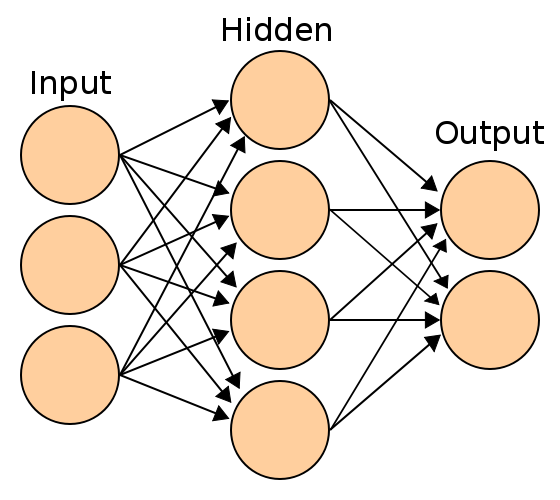
\includegraphics[width=4cm]
			{dnnBase}}
		\caption{\label{fig:dnnBase} Example of a Neural Network}
	\end{figure}

	 A DNN architecture is defined by its neurons, as in Figure \ref{fig:dnnBase}.  Each neuron in a layer uses the same activation function but has a distinct weight; this weight is the parameter learned during training. A DNN needs at least an input layer and an output layer. For this project, the output layer used is a softmax layer. For $n$ classes, a softmax generates an $n \times 1$ vector with an entry corresponding to the likelihood an input belongs to a respective class. The highest likelihood is then taken as the label.
	 
	 To implement and train the neural network, the Python Keras library was used. Keras offers easy to use graphics hardware acceleration which improves computation time allowing for more expensive optimizations to be trialed.
\subsection{Optimization Process}
	Neural network optimization aims to improve overfitting or underfitting of data. A systematic approach was taken to optimization. Parameters of the network were defined, and a range of values was determined for each parameter. One at a time, each parameter would be changed in its range and the network would retrain while all other parameters were kept at their baseline value. The UAR differential with the baseline network is recorded and the experiment is repeated. The baseline values were selected based on the standards in research and a range slightly above and, if possible, below was used.
	\begin{table}[!hbt]
		\centering
		\caption{Parameter Ranges and Baselines}
		\begin{tabular}{|c|c|c|}
			\hline
			Parameter     & Range       & Baseline \\ \hline
			Hidden Layer  & 1-4         & 1        \\ \hline
			Neuron Count  & 10-100      & 10       \\ \hline
			Epoch Count   & 10-100      & 30       \\ \hline
			Batch Size    & 10-125      & 30       \\ \hline
			Optimizer     & SGD or Adam & SGD      \\ \hline
			Learning Rate & 0.001-0.03  & 0.01     \\ \hline
			Feature Count & 5 or 100    & 5        \\ \hline
			Dropout       & 0-0.5       & 0        \\ \hline
		\end{tabular}
	\label{params}
	\end{table}

	The parameters can be broken down into two categories; architecture based and learning based. Hidden layer count, feature count and dropout fall in the architecture based and the remainder in the learning based.  The effects of both categories are observed and discussed in the results section.
\subsection{Loss Function}
	The goal of a loss function is to provide a numerical value to represent the loss or cost of a classification algorithm during training. In this project, the classification made must be the correct emotion as close as possible, so a function that punishes mislabeling heavily is favored. The cross entropy (CE) function is one such function; it is designed to be high cost if the probability of the prediction $y_p^k$ is not close to 1 for the index of its actual class value $y_a^k$. The function is defined as follows;
	\begin{equation}
	CE(y_p,y_a) = - \sum_{1}^{n}y_a^k \log y_p^k
	\end{equation}
	where $y_p$ is a vector containing the likelihood probability of each class is $y_a$ is a zero vector containing a 1 in the index of its labeled class. Because of $y_a$ only having one element that is not zero, the only value calculated by CE is the negative log of the likelihood of the predicted class being the correct class.
	
	CE was problematic during testing because it suffered in performance with the imbalance of classes. More than 80\% of the samples belong to one class, so more than 80\% of the loss function calculations will be aiming to fit one class. This results in the classifier fitting all data into the one overpopulated class. A simple solution to this problem was using weighted cross entropy (WCE). Calculated similarly to cross entropy, weighted cross entropy takes into account the weight $w$ of each class, giving more value to an individual prediction in a low sampled class versus an overpopulated class. This is calculated as follows;
	\begin{equation}
	CE(y_p,y_a, w) = - \sum_{1}^{n}w^k * y_a^k \log y_p^k
	\end{equation}
	
	